\documentclass[english,onecolumn]{article}
\usepackage[T1]{fontenc}
\usepackage{listings}
\usepackage{hyperref}
\usepackage{tabularx}
\usepackage{multirow}
\usepackage{tikz-timing}
\usepackage{graphicx}
\usepackage[style=ieee, backend=biber]{biblatex}

\definecolor{darkgreen}{HTML}{008000}
\lstset{frame=single,
    language=Haskell,
    breaklines=true,
    showspaces=false,
    showstringspaces=false,
    showtabs=false,
    commentstyle=\color{darkgreen},
    keywordstyle=\color{blue},
    stringstyle=\color{purple},
    title=\lstname}
\def\tabularxcolumn#1{m{#1}}
\pagenumbering{roman}
\tikzset{timing/draw grid}
\addbibresource{references.bib}

\begin{document}
\title{H2V --- Design Specification}
\author{Reuben D'Netto}

\maketitle
\tableofcontents{}
\pagebreak{}
\pagenumbering{arabic}

\section{Project Overview}
\subsection{Project Definition \& Objective}
H2V is a Haskell to Verilog compiler. The high-level objectives of this project are:
\begin{itemize}
\item to design and implement a compiler capable of generating equivalent Verilog from a program written in a subset of Haskell
\item to demonstrate the benefits of generating Verilog from Haskell compared to C
\end{itemize}

\subsection{Haskell}
% what is Haskell, and why use it?
Haskell is a purely functional language functional language with lazy evaluation.
This may be contrasted with C, which is an imperative language with strict evaluation.
The following sections discusses the differences between these languages, and the implications for generating logic.

\subsection{Comparison to C}
\subsubsection{Functional vs. Imperative Paradigms}
% functional vs imperative; C uses the wrong paradigm. Enables data-level parallelism
Haskell is a purely functional language; the result of each function is defined purely in terms of its inputs. All variables are immutable, and there is no global state. This may be contrasted with C, which is an imperative language; the program is defined in terms of instructions, most of which alter the program's state. This is demonstrated in the following example:

\begin{lstlisting}[language=C, caption={XORing an array in C.}, label={lst:xorC}]
int* xorArray(int mask, int* input, int* output, int N){
    for(int i = 0; i < N; i++){
        output[i] = input[i] ^ mask;
    } //end for

    return output;
}
\end{lstlisting}

\begin{lstlisting}[caption={XORing an array in Haskell.}, label={lst:xorH}]
xorArray :: Int -> [Int] -> [Int]
xorArray mask input = map (xor mask) input
\end{lstlisting}

In this example, we define a function which XORs each element of an input array with an argument called \textit{mask}. The C function iterates over the contents of the array, setting each value in sequence. The values of \textit{i} and \textit{output[i]} change throughout the function's execution; it is stateful. In contrast, the Haskell function is declarative; it defines the result to be a list of the same length as \textit{input}, where each element is the result of applying the function \textit{xor mask} to the corresponding element from \textit{input}. Note that there is no state, and that we have not defined an order in which the elements are computed.

\begin{tabular}{|c|c|c|c|c|c|c|c|c|c|c}
\cline{1-1} \cline{3-3} \cline{5-5} \cline{7-7} \cline{9-9}
& \multirow{4}{*}{$\longrightarrow$} & $x_0$ & $\longrightarrow$ & XOR & $\longrightarrow$ & $y_0$ & \multirow{4}{*}{$\longrightarrow$} & \\
\cline{3-3} \cline{5-5} \cline{7-7}
List & & $x_1$ & $\longrightarrow$ & XOR & $\longrightarrow$ & $y_1$ & & List \\
\cline{3-3} \cline{5-5} \cline{7-7}
Reader & & $\vdots$ & $\longrightarrow$ & $\cdots$ & $\longrightarrow$ & $\vdots$ & & Writer \\
\cline{3-3} \cline{5-5} \cline{7-7}
& & $x_N$ & $\longrightarrow$ & XOR & $\longrightarrow$ & $y_N$ & & \\
\cline{1-1} \cline{3-3} \cline{5-5} \cline{7-7} \cline{9-9}
\end{tabular} 

C is often informally referred to as portable assembly; it offers a similar degree of control to assembly over the processor without being limited to a specific instruction set. While this is desirable when compiling to machine code, it is extremely limiting when compiling to a hardware description language (HDL) such as Verilog.
The reason for this is that C is designed to express sequential computation, which is most easily expressed in terms of steps which mutate some global or local state. However, the primary advantage of HDL is that the resulting logic executes in \textit{parallel}. In the context of parallel computation, shared state becomes a bottleneck which limits throughput.
It is non-trivial to determine from Listing \ref{lst:xorC} whether one iteration of the loop depends on the execution of previous iteration, since it is unknown if the input and output arrays overlap.%
\footnote{C2H has qualifiers \cite[72]{C2H_UG} which may be used to state this explicitly, but the need for these increases the difficulty of use.}
Note that while there are few real--world scenarios where arrays would be aliased, C2H handles structures in the same way, \cite[54]{C2H_UG} and it is not uncommon for structures to contain pointers which alias like this.
To avoid these issues, C2H simply generates a state machine which executes each iteration sequentially.\cite[17]{C2H_UG}

The above limitation does not apply to Haskell; because the result of the function is defined purely in terms of its inputs, it is trivial to interpret the function such that the mapping operation is applied to multiple elements at once, enabling significant increases in throughput.
This is demonstrated in \ref{s:pipeline}.

\subsubsection{Side-effects}
The mutation of global state in the course of computing a result is referred to as a \textit{side-effect} in functional programming. C functions often rely on side-effects, which limit their parallelism and can introduce bugs. Consider the following:
\begin{lstlisting}[language=C, label={lst:side-effect}]
int y = 0;

int foo(int x){
    return (x > 0 || x < y++) ? 1 : 2;
}
\end{lstlisting}

The incrementing of \textit{y} in the condition is a side-effect of \textit{foo}. This means that multiple instances of \textit{foo} cannot be called in parallel, since they all depend on shared, global state.

Listing \ref{lst:side-effect} is particularly interesting because it also demonstrates a limitation of C2H. || is a short-circuit boolean operator; its second argument should not be evaluated if its first is true.\cite[s 6.5.14]{c_std}
C2H does not comply with this, evaluating both arguments.\cite[128]{C2H_UG}
This decision was likely made for performance reasons, but means that C2H effectively uses a dialect of C that is syntactically compatible with ANSI C but functions differently.
In contrast, because Haskell functions are stateless, the same problem cannot arise with H2V. In fact, expressions which do not directly contribute to the result of a function can be discarded completely, enabling optimizations that otherwise be complex to achieve.

\subsubsection{Memory Access and Pipelining}
\label{s:pipeline}
The single greatest limitation of C2H is C's reliance on pointers to pass arrays. This is because every array access is mapped directly to a single-port Avalon bus slave.\cite[54]{C2H_UG} In other words, within any given function, only one element of an array can be accessed at once, and that access will multiple clock cycles as the value must be written directly to the underlying SRAM/DRAM.
The same is true of global and static variables,\cite[55]{C2H_UG} and even assignments to local variables are registered, requiring a full clock cycle for each one.\cite[53]{C2H_UG}
There is also no support for inlining functions, which means that refactoring common functionality into a separate function will result in an additional overhead.\cite[53]{C2H_UG}
While this enables pipelining, it is excessive and significantly increases the latency of computing a single result.

H2V uses a completely different approach. Results are computed in purely combinatorial logic by default to maximise the amount of computation per clock cycle. In the future, registers will be inserted automatically to reduce the maximum propagation delay and enable pipelining. Where arrays are used (e.g. Listing \ref{lst:xorH}), multiple values will be read simultaneously, and intermediate values will be stored in registers to avoid the increased latency of memory access.

Consider Listing \ref{lst:arrayC}, which computes the pairwise difference of the elements of an array.
(Assume this function is an intermediate step in a computation, such that its data source and sink are other functions rather than RAM.)
Even with pipelining, no more than one subtraction will be performed per cycle, since C2H uses a single-port Avalon Memory bus for array access. This reflects the imperative structure of the code; the loop's iterations may be pipelined together, but remain in sequence.

\begin{lstlisting}[language=C, caption={Array Bottleneck Example (C).}, label={lst:arrayC}]
    void diff(int *array, int n){
        for(int i = 0; i < (n - 1); i++)
            array[i] = array[i+1] - array[i];
    }
\end{lstlisting}

In contrast, Listing \ref{lst:arrayH} takes a more functional approach.
\textit{zipWith} returns a list whose n\textsuperscript{th} element is the result of applying a function to the n\textsuperscript{th} elements of two lists, up to the last element of the shorter list. We specify subtraction as the function to be applied, and use the \textit{tail} function (which converts \textit{xs[0..N]} into \textit{xs[1..N-1]}) to offset the list by one element.
Since each element is defined independently of the others, multiple elements in the result can be computed simultaneously.

Although the current list protocol currently only supports reading one element at a time,\footnotemark extending it to allow multiple elements to be read/written at once is trivial.
\footnotetext{See \ref{s:lists}.}

\begin{lstlisting}[caption={Array Bottleneck Example (Haskell).}, label={lst:arrayH}]
    diff :: [Int] -> [Int]
    diff xs = zipWith (-) (tail xs) xs
\end{lstlisting}

\subsection{Verilog}
% what kind of Verilog we generate
\subsubsection{Nios accelerators}
The primary application of H2V will be the generation of Nios accelerators. A Nios Custom Instruction Slave can be generated to encapsulate the generated Verilog, allowing Haskell functions to be called from C code running on the Nios processor.
This has the advantage of enabling the user to write computational code in Haskell, while still using C where it is more convenient.

\subsubsection{Recursive Functions}
H2V will be capable of generating Verilog modules from tail-recursive functions. A tail-recursive function is one which returns the  result of a call to itself when it recurses. e.g. Listing \ref{lst:tailrec}. Tail-recursive functions can be evaluated in a constant amount of memory, as they do not require a call stack. The ability to compile tail-recursive functions is especially important, as they replace loops in functional languages.

\begin{lstlisting}[language=C, caption={An example of a tail-recursive function in C.}, label={lst:tailrec}]
int absDiff(int x, int y){
    return (x < y ? absDiff(y, x) : x - y);
}
\end{lstlisting}

Recursive functions will be compiled into two modules --- one encapsulating the combinatorial logic, and one the synchronous logic.
The inputs will be written to registers, and then overwritten on each recursion. The combinatorial module will output the new values for the registers, a result, and a signal indicating whether the call has terminated. It may also implement the same interface as other functions (see \ref{s:functionInterface}), if support for nested recursive functions is implemented.
This approach means that loop unrolling can be implemented easily for functions with simple combinatorial stages.

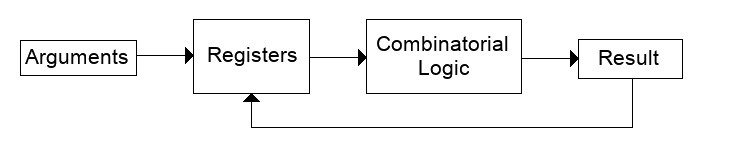
\includegraphics[scale=0.5]{./recursive.png}

\subsubsection{Pipelining}
At present, H2V translates all non-recursive functions to purely combinatorial logic. This minimizes the no. of cycles a function will take to evaluate, at the cost of a significantly lower upper bound on clock frequency. One optimization that could be made to this would be to insert buffers in long sections of combinatorial logic. The buffers' positions could be determined using the propagation delay of each operation, which would allow us to increase the upper bound on the clock frequency while using only a minimum no. of registers and additional clock cycles.

\subsubsection{Direct Memory Access (DMA)}
\label{s:DMA}
% DMA - sequential vs random, read vs write
The generated Verilog will support accessing memory via the Avalon Memory bus. Sequential access in Haskell will be provided via lists.
Memory access will only be performed when reading from or writing to top-level function arguments. Code within the accelerator will store intermediate values in registers, or generate them on demand.\footnote{See \ref{s:lists}.}

\subsection{Additional Output}
To facilitate the use of generated Nios accelerators, QSys peripheral templates and C header files can also be generated to simplify calling the accelerator from C code.
A visual representation of the source code's data flow will also be generated to aid debugging.

\section{Equipment}
\subsection{Development Tools}
Development of H2V will use the Glasgow Haskell Compiler, which is freely available online.

\subsection{Target Platform}
H2V is intended to run on a standard desktop computer. A copy of Altera Quartus 12.0 will be required to synthesize the generated accelerator. It has been tested with the Altera Cyclone II/IV FPGAs, though it should be compatible with any FPGA supported by Quartus.

\section{Design}
\subsection{Compilation Process}
\subsubsection{Lexical Analysis \& Parsing}
\paragraph{Parsing}
The source code is parsed using the \textit{haskell-src} library.%
\footnote{See http://hackage.haskell.org/package/haskell-src}
This produces an Abstract Syntax Tree (AST), a complex tree structure which contains all expressions and declarations found in the source code. Syntactically meaningless features of the source code, such as comments, whitespace, etc. are discarded.

\paragraph{Cleaning}
To simplify the generation of the Data Flow Diagram (DFD), the AST is then '\textit{cleaned}'. i.e. it is rewritten to use a minimal subset of the available expressions and declarations. Infix application is converted to prefix application, certain operators are replaced by built-in function calls, and functions with multiple matches or pattern binding are rewritten as a single match with \lstinline{if} and \lstinline{let} statements.

\subsubsection{DFD Generation}
\paragraph{DFD Creation}
Each expression is converted to a data flow node. Declarations are sorted (to resolve data dependencies), converted to nodes, and pushed onto a stack to facilitate their resolution by other expressions. All nodes are assigned unique numeric identifiers.

\paragraph{Closure Rewriting}
Haskell allows nested functions to use values and arguments defined in their parent function. As nested functions are mapped to modules independent of their parent function, the values closed over must be conveyed to them in the form of additional arguments.
All references to the function must then be updated to pass these values as arguments.

\begin{lstlisting}[caption={A nested function with a closure.}, label=lst:closure]
f1 :: Int -> Int
f1 x = z where
    y = x + 1
    z = f2 x

    f2 :: Int -> Int
    f2 a = a * y
\end{lstlisting}

\begin{lstlisting}[caption={The function from Listing \ref{lst:closure}, rewritten to use arguments.}]
f1 :: Int -> Int
f1 x = z where
    y = x + 1
    z = f2 y x

    f2 :: Int -> Int
    f2 yc a = a * yc
\end{lstlisting}

\paragraph{Linking}
For each scope containing functions, templates of all functions are pushed onto the namespace stack before they are converted. This is necessary so that recursive functions are able to resolve themselves. Once all functions have been converted to DFD subgraphs, all references to the templates are replaced with the resulting DFDs.

\subsubsection{Verilog Generation}
The DFD is transformed into a Verilog file. Each function is converted into a module, and each node into a wire or register. All expressions use either built-in operators or function/module calls. Wrapper logic is generated for recursive functions, lists, etc.

\subsection{Design of Generated Verilog}
\subsubsection{Function Interface}
\label{s:functionInterface}
All functions will be defined with the following interface:

\begin{tabularx}{\textwidth}{|c|c|c|X|}
\hline 
Name & Type & Width (bits) & Description \\ \hline 
Arguments & Input & Variable & Arguments used by the function to compute its result. \\ \hline 
Result & Output & Variable & The result of evaluating the function. \\ \hline 
Clock & Input & 1 & The clock signal used for the accelerator. This should be the same clock used by the Avalon buses. \\ \hline 
Ready & Input & 1 & Asserted high when the arguments are valid. \\ \hline 
Done & Output & 1 & Asserted high when the result is valid. \\ \hline
\end{tabularx} 

Computation of a synchronous function will begin when \textit{Ready} is asserted high, and signal its completion by driving \textit{Done} high. \textit{Ready} should remain high for the duration of the computation. If \textit{Ready} is unasserted at any point, the module will be reset. Combinatorial functions should pass these signals through to any functions they call. Combinatorial functions without function calls (i.e. leaves in the function call graph) should assign \textit{Done} to \textit{Ready}.

\begin{tikztimingtable}[scale=2, line width=1]
    Clock & 9{C} \\
    Ready & L6H2L \\
    Arguments & U6D{}2U \\
    Done & 3L4H2L \\
    Result & 3U4D{}2U \\
\end{tikztimingtable}

This definition ensures that synchronous and combinatorial functions can be called in the same manner, and enables speculative evaluation. E.g. Given a ternary expression \lstinline[language=C]{(c ? t : f)}, the computation of all three terms can be initiated at the same time, and the evaluation of the unused term aborted once \textit{c} has been computed.

Note that the signals for arguments and results are a simplification --- if one of the arguments is a list, additional signals will be added (see \ref{s:lists}).

\subsubsection{Lists}
\label{s:lists}
Haskell uses linked lists for the representation of ordered sequences of data. This is a convenient model for representing streams of data, especially when combined with lazy evaluation, as this allows functions to consume the head of the list while the tail is still be generated.

Where a list is returned, the following signals shall be used to encapsulate access to it:

\begin{tabularx}{\textwidth}{|c|c|c|X|}
    \hline 
    Name & Type & Width (bits) & Description \\ \hline 
    Request & Input & 1 & Advance to the next element of the list. \\ \hline 
    Acknowledge & Output & 1 & Asserted high when the next element of the list is available, or Empty has been asserted. \\ \hline
    Head & Output & Variable & The value of the element at the head of the list. Only valid if Empty is false, and Acknowledge is true. \\ \hline 
    Empty & Output & 1 & True if there are no more elements in the list. \\ \hline 
\end{tabularx} 

Note that this is a synchronous interface; the clock signal is taken from the function which computes the values in the list.
The list can only be accessed as long as the function has \textit{Ready} asserted high.
If \textit{Request} remains high in the clock cycle after \textit{Acknowledge} is asserted, it will be interpreted as a second request.
\textit{Head} will be valid for the first cycle \textit{Acknowledge} is asserted, and will remain valid until \textit{Request} is asserted.

\begin{tikztimingtable}[scale=1.5, line width=1]
    Clock & 21{C} \\
    Request & L1{4H2L}1{6H2L}1{4H2L} \\
    Acknowledge & 1{L}1{2L2H2L}1{2L4H2L}1{2L2H2L} \\
    Empty & U2U2L4U4L4U4H \\
    Head & 3U2D{A}4U4D{B}8U \\
\end{tikztimingtable}

The list interface does not support indexing, although it can be emulated through repeated requests.\footnotemark Once an element has been advanced past, its value is discarded. As a consequence of this, if multiple values from a list are required they will need to be buffered by the calling function.
\footnotetext{This is consistent with the behaviour of the indexing operator in Haskell, which has a time complexity of O(N).}

Lists may have infinite length. This interface may be extended in the future to allow multiple values to be read in one clock cycle.

\subsubsection{Direct Memory Access}
%TODO: I should probably have something more here...
DMA will be implemented using the Avalon Memory bus. See \ref{s:DMA} for details.

\section{Current State}
% description of what has been done, and what remains
% comparison with requirements analysis
% QUESTION: will we have time for Nios integration? Might be better to focus on general purpose compilation and optimizations
The following section discusses the current state of H2V, and discusses which requirements have been satisfied thus far.
References to specific requirements will use the same numeric identifier as in the requirements analysis, prefixed by one of the following designations:

\begin{description}
        \item[REQ] Hard requirement.
        \item[OF] Optional feature.
        \item[ASS] Assumption.
        \item[LIM] Limitation.
\end{description}

\subsection{Compiler}
\paragraph{Requirements}
The compiler is able to generate combinatorial Verilog modules (REQ 3.1.1.1).
Function calls are supported, but tail-recursion is not available yet (REQ 3.1.1.1b).
The function interface discussed in \ref{s:functionInterface} has not been implemented yet.
Once tail-recursion has been completed,\footnotemark the hard requirements for this section will have been met.
\footnotetext{This is expected to be ready within a week.}

\paragraph{Optional Features}
The language compiled is a strict subset of Haskell (OF 3.1.2.1). A protocol definition has been created for lists and first-class functions (OF 3.1.2.2).%
\footnote{First-class functions are merely functions passed as arguments. They can therefore be implemented by passing the signals defined in \ref{s:functionInterface}, similar to how a list is passed.}
The design of recursive functions allows for loop vectorization (OF 3.1.2.5), however this has not been been implemented yet.

Support for multiple source files (OF 3.1.2.4) and type inference (OF 3.1.2.7) have not been implemented, but remain feasible. Support for unary non-tail recursive functions with bijective tail expressions (OF 3.1.2.3) is unlikely to be implemented.

\subsection{QSys Integration}
None of the requirements in section 3.2 have been implemented yet.
As C headers and QSys component definitions can easily be written by hand, they are of low priority compared to other sections. e.g. section 3.3. Should other requirements take longer to implement than anticipated, these requirements may be discarded.

\subsection{Direct Memory Access}
DMA has not been implemented yet (REQ 3.3.1). It is scheduled to be completed immediately after tail-recursion (REQ 3.1.1.1b). 
Sequential read (REQ 3.3.1) and write (OF 3.3.2.1) access with naive caching (OF 3.3.2.4) is expected to be completed on schedule. 
Due to the design of the list protocol,\footnote{See \ref{s:lists}.} memory access may now exceed one clock cycle. (ASS 3.3.3.1 --- no longer applies)

Random access (OF 3.3.2.2, OF 3.3.2.3) is not currently planned.

\subsection{Performance}
Implementations of certain use cases have been written in Haskell for the purposes of testing the compiler, however no benchmarks have been conducted at this point in time (REQ 3.4.1.1). Currently, the focus of the project is on implementing critical features, as opposed to refining their performance. Work on these requirements is expected to comment mid-semester two.

\subsection{Legal}
The haskell-src library used for parsing is licensed under the three clause BSD license, which does not restrict the license derivative works are published under. There are therefore no impediments to publishing the project under a free software license at this point in time (REQ 3.5.1).

\appendix
\lstset{basicstyle=\footnotesize}

\section{Appendix --- Examples}
The following section contains examples of Haskell source code that can be compiled by H2V into DFDs and Verilog.

\subsection{Declaration Resolution}
This example demonstrates the resolution of terms whose values depend on others defined later within the same scope.

\lstinputlisting[firstline=7, lastline=11]{../../H2V/test.hs}
\includegraphics[scale=0.25]{./examples/f1.png}
\lstinputlisting[language=Verilog]{./examples/f1.v}

\subsection{Nested Functions \& Closures}
This example demonstrates the use of nested functions which close over values defined in the parent function.
Note that as closure rewriting is not fully implemented yet, there are edges between nodes defined in different subgraphs (functions).
This will be resolved in the near future by converting closure values into additional arguments.

\lstinputlisting[firstline=13, lastline=19]{../../H2V/test.hs}
\includegraphics[scale=0.25]{./examples/f2.png}
\lstinputlisting[language=Verilog]{./examples/f2.v}

\subsection{Tail--Recursion}
This example demonstrates a nested, tail--recursive function.
All leaf expressions in \textit{fib'} are either combinatorial values or a call to itself.
Verilog cannot currently be generated for recursive functions due to a bug in H2V.

\lstinputlisting[firstline=21]{../../H2V/test.hs}
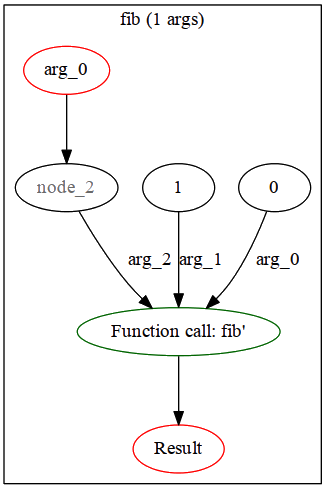
\includegraphics[scale=0.25]{./examples/fib.png}

\section{Appendix --- Source Code}
\lstinputlisting{../../H2V/main.hs}
\lstinputlisting{../../H2V/Common.hs}
\lstinputlisting{../../H2V/DfdDef.hs}
\lstinputlisting{../../H2V/GenerateDFD.hs}
\lstinputlisting{../../H2V/RenderGraphviz.hs}
\lstinputlisting{../../H2V/RenderVerilog.hs}
\lstinputlisting{../../H2V/AST_Display.hs}

\printbibliography

\end{document}
